
\chapter{Data}\label{ch:data}

The data set $X = \{(x^{(1)}, y^{(1)}), (x^{(2)}, y^{(2)}), \ \dots\}$ consists of audio samples,
sequences of spectral input features $x^{(i)}$, and the corresponding transcript
composed of the character sequence $y^{(i)}$ (Chapter~\nameref{ch:background}).
The vast dataset is crucial to achieving the exceptional performance of speech recognition systems,
especially in the case of the systems based on a deep neural network.
The model tries to identify patterns presented in a dataset.
Therefore the corpus must be of high quality because the model can easily adapt
to anomalies or particular characteristics of the training dataset.
We analyze the corpus with particular care before starting to work with our models.
The data defines which model architecture is the most convenient.


\section{Audio Representation}\label{sec:audio-representation}

Audio samples have the single-channel (mono) with the sampling rate of 16 kHz and the depth of 16 bits.
Input data $x^{(i)}$ to the model is the audio signal presented in the form
of the \textit{Mel-scale~log~filter~banks} (however also the use of the raw speech is presented in~\cite{zeghidour2019}).
In this representation, the energy in the individual bands of the spectrogram
is scaled using the \textit{mel~scale}.
The use of more sophisticated representations such as \textit{Mel~Frequency~Cepstral~Coefficients} (\textit{MFCC})~\cite{sahidullah2012}
does not yield noticeable improvements, so we deem additional transformations as needless.
The table~\ref{table:data-features} shows the \textit{Mel-scale~log~filter~banks} transformation parameters,
which gives the best results for the Polish language.

\begin{table}[h!]
\vspace*{10pt}
\centering
 \begin{tabular}{c c c c c c}
  \toprule
  Pre-emphasis & Winlen (ms) & Winstep (ms) & Winfunc & NFFT & Filterbanks \\
  \midrule
  0.95  &  25  &  10  & hamming & 512 & 80
  \bottomrule
 \end{tabular}
\caption{
The transformation parameters: the pre-emphasis coefficient, the window length, the step size,
the window function, the DFT size, the number of filterbank energies.
}
\label{table:data-features}
\end{table}

The dataset is normalized so the energy level for each sample remains constant.
For each \textit{filter bank} in the \textit{train} dataset, we calculate the global
average and standard deviation.
Then base on these statistics, we normalized the \textit{train}, the \textit{dev} and the \textit{test} datasets.
Alternatively, one can use the \textit{Batch Normalization} as the first model layer
to achieve a similar behaviour~\cite{ioffe2015}.
However, a large dataset is often highly inconsistent, so the statistics ($\mu, \sigma$)
vary considerably for different batches.
In consequence, the model is subjected to the strong regularization, which in our experiments negatively
affects the model's performance.


\section{Dataset Construction}\label{sec:dataset-construction}

The vast majority of transcribed audio datasets are closed, and those concerning the Polish language in particular.
One of the few publicly available datasets is the \textit{Clarin-PL}~\cite{korzinek2017},
created by the European initiative the \textit{Common Language Resources and Technology Infrastructure} (Clarin)~\cite{varadi2008}.
The polish fragment \textit{Clarin-PL} is small (36 hours), but in our work
we use additionally the closed dataset \textit{Jurisdic}~\cite{demenko2008} which is over 10 times
larger than the~\textit{Clarin-PL}.
Both the \textit{Clarin-PL} and the \textit{Jurisdic} are well documented,
and contain a variety of recording sources, including the \textit{read speech},
the \textit{spontaneous dictation}, and the \textit{phone calls}.

\begin{figure}[!h]
    \centering
    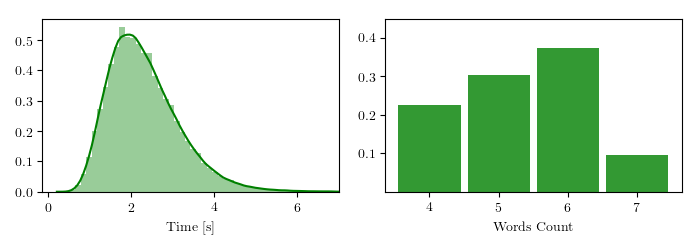
\includegraphics[width=13cm]{figures/data-histogram.png}
    \caption{
Histograms of the samples from the training dataset aggregated according to: the length of samples (left)
and the number of words (right).}
    \label{fig:data_histograms}
\end{figure}

The data comes from a variety of sources is highly non-uniform, both in terms of audio data and transcriptions.
The number of words in recordings ranges from one to several dozen.
Therefore, we perform the segmentation of samples into single words on both corpora, and then
combine into utterances from 4 to 7 words.
In consequence, the model is not able to recognize longer dependencies (more than 7 words),
which is a reasonable assumption in the context of this work.
However, the samples are more homogeneous, and the number of observations is increased significantly.
The figure~\ref{fig:data_histograms} shows the distribution of samples by the length of recordings,
and the number of words in the transcription after segmentation.

\begin{table}[h]
\vspace*{10pt} 
\centering
 \begin{tabular}{l c c}
  \toprule
  Corpus & Size (hours) & Samples (k) \\
  \midrule
  Clarin-PL (train) & 34  & 41 \\
  Jurisdic & 351 & 578 \\
  \bottomrule
 \end{tabular}
\caption{
The components of the training dataset.
The number of samples contains from 3 to 7 words (after the segmentation).
}
\label{table:train_dataset}
\end{table}

The dataset \textit{Clarin-PL} is divided into 3 parts the \textit{train}, the \textit{dev}, and the \textit{test}.
The proportions of the division are as follows 80\%, 10\%, and 10\%.
Each part has independent speakers and unique transcriptions.
The data from the corpus \textit{Jurisdic} do not appear in the \textit{dev} and the \textit{test} datasets,
because most transcriptions (82\%) are duplicated (details how it was built can be found in~\cite{demenko2008}).
The figure~\ref{fig:data_repetitions} shows the distribution of the duplicated transcriptions
in the training dataset.
Speech recognition systems \textit{end-to-end} learn to recognize \textit{phonemes} parallel
to learning the language model.
In this case, the language model has a strong \textit{bias} towards repetitive words.
The knowledge included in the much larger \textit{Jurisdic} corpus is important, so it is
entirely included into the training dataset (table~\ref{table:train_dataset}).

\begin{figure}[!h]
    \centering
    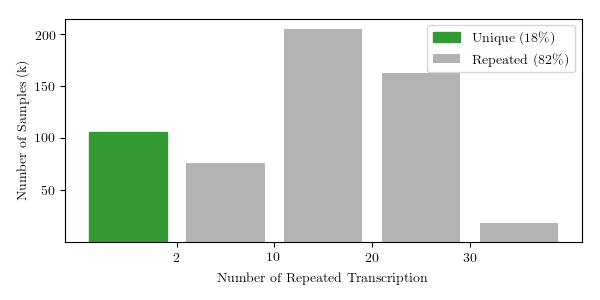
\includegraphics[width=10cm]{figures/data-repetitions.png}
    \caption{
The distribution of the number of transcription repetitions in the training dataset.
Samples with the unique transcript are marked in green.
The grey color represents the samples in which transcriptions are repeated.
}
    \label{fig:data_repetitions}
\end{figure}


\subsection*{Synthetic Dataset}
In this work, we present a model that derives language knowledge from synthetic data.
For this purpose, we generate the auxiliary synthetic corpus of over ten thousand hours.\footnote{
Unfortunately, due to the limited duration of the research, we have only used a part of the synthetic corpus.
}
Due to the high accessibility, we choose a commercial \textit{Text To Speech}~(\textit{TTS}) model.
The system based on the \textit{WaveNet}~\cite{oord2016} generated files based on transcripts created from the publicly
available text corpus \textit{PolEval}~\cite{ogr:kob:18:poleval}.
All transcriptions are composed of 7 consecutive correct tokens, not including punctuation marks.\footnote{
A token is a string of contiguous characters between two spaces, or between a space and punctuation marks.
The correct token means that it is constructed only from chars available in the model alphabet $\ell$.
}
The created synthetic speech corpus is publicly available.


\section{Data Augmentation}\label{sec:data-augmentation}

The data augmentation is a strategy that enables to increase the diversity of data available for training significantly.
Most of the augmentation methods in speech recognition systems operate directly on audio data~\cite{kanda2013,ragni2014,ko2015}.
The different approach \textit{Spec~Augment}~\cite{park2019} is the augmentation method which operates on the transformed features,
for instance, the spectrogram bands.
The method is simple and based on three stages: wrapping the features, masking blocks of frequency channels,
and masking blocks of time steps.
In this work, we use the last two parts that have a definite impact on the results and can be applied
with a low computing cost.
The sample masking makes the model more resistant to distortion and
fading of information both in the time and frequency domain.
The figure~\ref{fig:data_augmentation_1} shows an example of augmentation.

\begin{figure}[!h]
    \centering
    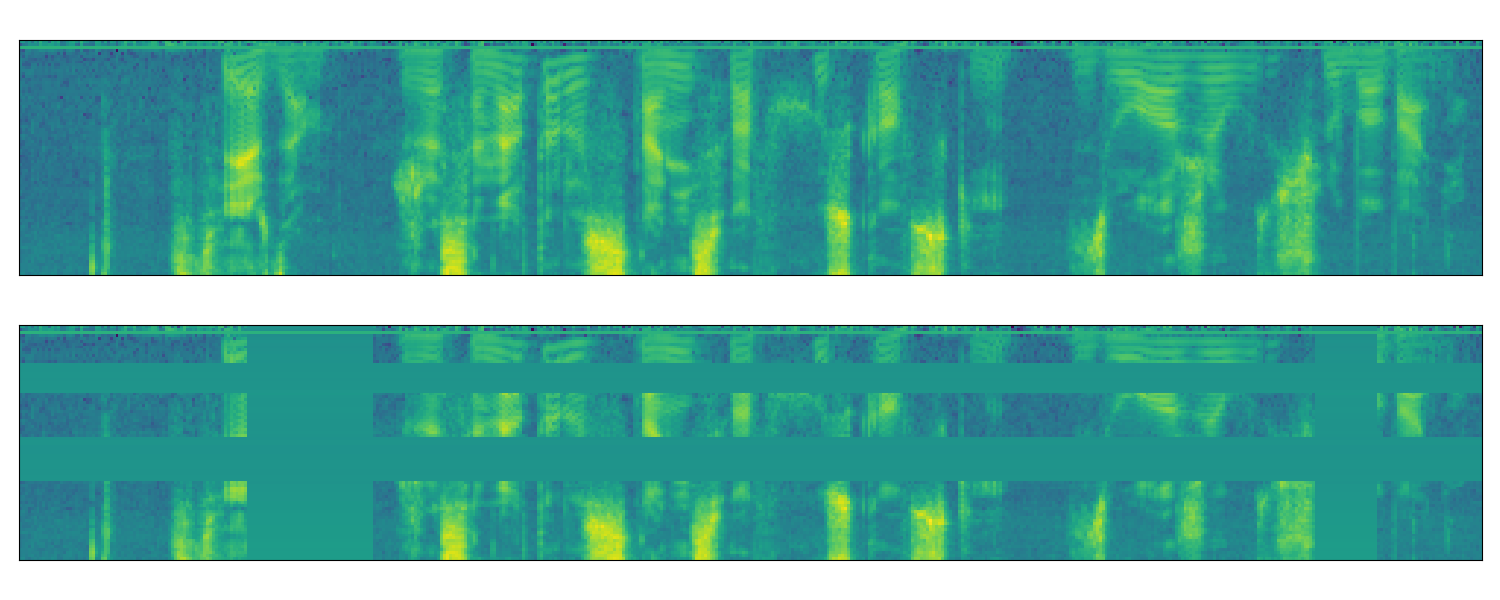
\includegraphics[width=12cm]{figures/data-augmentation-1.png}
    \caption{
The example of augmentation of a 500-frame sample:
the original sample (top) and the sample after augmentation (bottom).
The parameters are respectively $m_f=2, F=20, m_t=2, T=50$.
}
    \label{fig:data_augmentation_1}
\end{figure}

High values of $T$ parameter shown in~\cite{park2019}, in the range from 50 to 100 frames,
mask a significant part of the word.
The augmentation method, masking long fragments of the audio, forces the model
to make a prediction based on the context of other words.
The technique of masking a fragment of input data is strongly associated with language
modeling strategies~\cite{mikolov2013,peters2018,howard2018,devlin2019}.
Unfortunately, in the case of inflected languages (including Polish), the proposed technique in the time domain
does not improve the performance.
Large masks (e.g. $T=100$) lead to the training instability, while smaller
ones (e.g. $T=20$) bring small benefits.

% TODO: change the pic
\begin{figure}[!h]
    \centering
    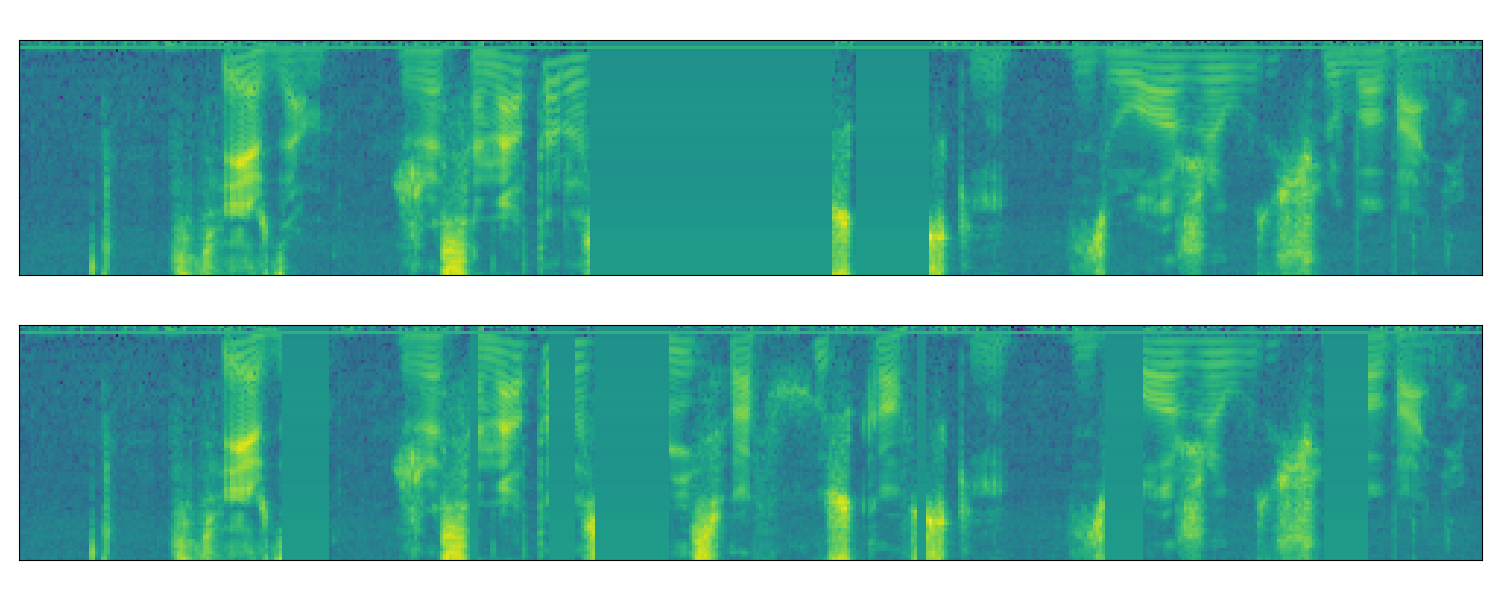
\includegraphics[width=12cm]{figures/data-augmentation-2.png}
    \caption{
The original augmentation method (top) with parameters $m_t=2, T=100$ and modified
(down) with parameters $T_{ratio}=0.1$, $T=<5.25>$, $T=10$.
The modified method is supposed to mask single phonemes rather than words, and prevent to overlap masks.
}
    \label{fig:data_augmentation_2}
\end{figure}

We adjust the data augmentation technique, in the time domain, to the specificity of the inflected language,
which requires more attention to words endings (figure~\ref{fig:data_augmentation_2}).
We have observed that we achieve better results when we use a few small masks.
In our case, the mask should try to cover single phonemes, not whole words.
The proposed augmentation technique is controlled by three parameters: $T$, $T_{ratio}$ and $T_{space}$.
The $T$ parameter specifies the range from which the mask width is drawn (\textit{uniform~distribution}).
The best results we obtain for the range $T=<5,15>$, which is correlated with the statistical length
of phonemes in Polish~\cite{igras2013}.
The $T_{ratio}$ parameter describes the ratio of masked parts to the entire sample.
The $T_{space}$ parameter specifies the minimum gap between masked sections.
Close (or overlapped) masks lead in our case to the training disruptions, because
the model is not able to handle large mask at all.
